%%%%%%%%%%%%%%%%%%%%%%%%%%%%%%%%%%%%%%%%%%%%%%%%%%%%%%%%%%%%%%%%%%%%%%%%%%%%%%%%%%%%%%%%%%
%                                 FORMATOS                                               %
%%%%%%%%%%%%%%%%%%%%%%%%%%%%%%%%%%%%%%%%%%%%%%%%%%%%%%%%%%%%%%%%%%%%%%%%%%%%%%%%%%%%%%%%%%
% \DeclareMathAlphabet{\mathpzc}{OT1}{pzc}{m}{it}
% \newtheorem{dfn}{Definition}
% \newtheorem{thm}{ Theorem}[section]
% \newtheorem{pro}{ Proposition}[section]
% \newtheorem{lem}{ Lemma}[section]
% \newtheorem{definition}{ Definition}[section]
% \newtheorem{corollary}{ Corollary}[section]
% \newtheorem{consequence}{ Consequence}[section]
% \newtheorem{remark}{ Remark}[section]
% \newtheorem{example}{\bf Example}[section]
% \newtheorem{proof}{\bf Proof}[section]
% \newproof{pf}{\bf Proof}
% 
% \newcommand{\fin}{\vrule height3pt width3pt depth2pt}
% \newcommand{\normL}[1]{\left[\mathbb{E}\left|#1\right|^2\right]^{1/2}}
% \newcommand{\ms}[1]{\mathbb{E}\left|#1\right|^2}
% \newcommand{\mep}[1]{\mathbb{E}|#1|^p}
% \newcommand{\m}[1]{\mathbb{E}#1}
% \newcommand{\meanp}[2]{\mathbb{E}\left|#1\right|^{#2}}
% \newcommand{\condexp}[2]{\mathbb{E}\left[#1|#2\right]}
% \newcommand{\lftrght}[3]{\left#2 #1\right #3}
% \newcommand{\revision}[1]{\textcolor{BrickRed}{#1}}
%%%%%%%%%%%%%%%%%%%%%%%%%%%%%%%%%%%%%%%%%%%%%%%%%%%%%%%%%%%%%%%%%%%%%%%%%%%%%%%%%%%%%%%%%%
%                                     TITLE                                              %
%%%%%%%%%%%%%%%%%%%%%%%%%%%%%%%%%%%%%%%%%%%%%%%%%%%%%%%%%%%%%%%%%%%%%%%%%%%%%%%%%%%%%%%%%%
%\begin {document}
%   \begin{frontmatter}
%     \title{
%       Convergence and asymptotic stability  of  the explicit
%       Steklov method for stochastic differential equations}
%     \author[sj]{Sa\'ul D\'{\i}az-Infante}
%     \author[sj]{ Silvia Jerez \corref{cor1}}
%     \address[sj]{
%       Department of Applied Mathematics, CIMAT, Guanajuato, Gto.,Mexico, 36240.
%      }
%     \cortext[cor1]{Corresponding author. Email address: jerez@cimat.mx.}
  %%%%%%%%%%%%%%%%%%%%%%%%%%%%%%%%%%%%%%%%%%%%%%%%%%%%%%%%%%%%%%%%%%%%%%%%%%%%%%%%%%%%%%%%
  %                                   ABSTRACT                                           %
  %%%%%%%%%%%%%%%%%%%%%%%%%%%%%%%%%%%%%%%%%%%%%%%%%%%%%%%%%%%%%%%%%%%%%%%%%%%%%%%%%%%%%%%%

%   \begin{keyword}
%     stochastic differential equations;
%     explicit methods; convergence; asymptotic stability;
%     BD simulation; logistic equation.
%   \end{keyword}
%   \end{frontmatter}
%%%%%%%%%%%%%%%%%%%%%%%%%%%%%%%%%%%%%%%%%%%%%%%%%%%%%%%%%%%%%%%%%%%%%%%%%%%%%%%%%%%%%%%%%%
%                            SECTION: Introduction                                       %
%%%%%%%%%%%%%%%%%%%%%%%%%%%%%%%%%%%%%%%%%%%%%%%%%%%%%%%%%%%%%%%%%%%%%%%%%%%%%%%%%%%%%%%%%%

%%%%%%%%%%%%%%%%%%%%%%%%%%%%%%%%%%%%%%%%%%%%%%%%%%%%%%%%%%%%%%%%%%%%%%%%%%%%%%%%%%%%%%%%%%
%                                 SECTION: Model                                         %
%%%%%%%%%%%%%%%%%%%%%%%%%%%%%%%%%%%%%%%%%%%%%%%%%%%%%%%%%%%%%%%%%%%%%%%%%%%%%%%%%%%%%%%%%%
  
   
%%%%%%%%%%%%%%%%%%%%%%%%%%%%%%%%%%%%%%%%%%%%%%%%%%%%%%%%%%%%%%%%%%%%%%%%%%%%%%%%%%%%%%%%%%
%SECTION:
%	Connsistency Converegence and non linear Stability
%%%%%%%%%%%%%%%%%%%%%%%%%%%%%%%%%%%%%%%%%%%%%%%%%%%%%%%%%%%%%%%%%%%%%%%%%%%%%%%%%%%%%%%%%%

%%%%%%%%%%%%%%%%%%%%%%%%%%%%%%%%%%%%%%%%%%%%%%%%%%%%%%%%%%%%%%%%%%%%%%%%%%%%%%%%%%%%%%%%%%

%%%%%%%%%%%%%%%%%%%%%%%%%%%%%%%%%%%%%%%%%%%%%%%%%%%%%%%%%%%%%%%%%%%%%%%%%%%%%%%%%%%%%%%%%%
  
  \section{Nonlinear stability} \label{sec5}
      To continue the stability analysis of the explicit Steklov method,  we now discuss
    the nonlinear case since a linear stable numerical stochastic method  does  not imply
    that is stable  under same conditions for any nonlinear problem. So, we study
    sufficient conditions for the nonlinear stability of the explicit stochastic method
    \eqref{Steklov} applied on the  autonomous SDE \eqref{eqn:autonomousSDE} in both
    multiplicative and additive cases.
    \subsection{Multiplicative Noise}
    Here  we prove the nonlinear asymptotic stability in a quadratic mean-square sense
    for the Steklov approximation.
    \begin{dfn}\label{dfn:SNMS}\cite{Baker2000a}
      Let $Y_n$ and $\widehat{Y}_n$ two different numerical recurrences  with
      corresponding initial process  $Y_0$ and $\widehat{Y}_0$. We shall say that a
      discrete time, $Y$ is numerically zero-stable in quadratic mean-square sense if given
      $\epsilon >0$, there  are positive constants $h_0$ and $\delta=\delta(\epsilon,h_0)$
      such that for all $h\in(0,h_0)$ and positive integers $n \leq T/h$ whenever
      $\ms{Y_0-\widehat{Y}_0}<\delta$ then
      \begin {eqnarray}\label{eqn:SNMS}
	\rho_n :=
	\ms{Y_n-\widehat{Y}_{n}}<\epsilon .
      \end{eqnarray}
      If the method is stable and $\rho_n \to 0$ when $n\to \infty$, then the method is
      asymptotically zero-stable in the quadratic mean-square sense.
    \end{dfn}
    In order to prove that the Steklov method satisfies the definition
    \ref{dfn:SNMS}, we will follow the idea of the proof given in
    \cite[Th.4]{Baker2000a}.
    \begin{thm}
      If the functions $\Psi_h$ and $G$ of the Steklov method \eqref{Steklov} are
      Lipschitz with constant $L$, then the Steklov method for the multiplicative SDE 
      \eqref{eqn:autonomousSDE} is zero-stable in quadratic mean square sense.
       In addition, if $L<1$ then the Steklov method is asymptotically zero-stable stable in quadratic 
       mean-square sense.
    \end{thm}
    \begin{Proof}
      Given two Steklov sequences $Y_n$ and $\widehat{Y}_n$ we have
      \begin{align*}
	\left(Y_{n+1}-\widehat{Y}_{n+1}\right)^ 2
	  &\leq
	  \left(
	    \Psi_h(Y_n)
	    -
	    \Psi_h(\widehat{Y}_n)
	  \right)^2 \\
	  &+
	  2\left(
	  \Psi_h(Y_n)
	    -
	  \Psi_h(\widehat{Y}_n)
	  \right)
	  \left(
	    G(Y_n)-G(\widehat{Y}_n)
	  \right)
	  \Delta B_n\\
	   &+
	  (G(Y_n)-G(\widehat{Y}_n))^2
	  (\Delta B_n)^2,
      \end{align*}
      for $0<n<N$ with $T=Nh$. Now, taking expected values conditioned on the
      $\sigma$-algebra $\mathcal{F}_{t_0}$ of the above inequality and applying
      properties of the conditional expectation we get
      \begin{align*}
	  \ms{Y_{n+1}-\widehat{Y}_{n+1}}
	  &\leq
	  \condexp{
	    \left|
	      \Psi_h(Y_n)
	      -
	      \Psi_h(\widehat{Y}_n)
	    \right|^2
	  }{\mathcal{F}_{t_0}}
	  \\
	  &+
	  2\left|
	  \condexp{
	    \left(
	      \Psi_h(Y_n)
	      -
	      \Psi_h(\widehat{Y}_n)
	    \right)
	  \left(
	    G(Y_n)-G(\widehat{Y}_n)
	  \right)
	  \Delta B_n}{\mathcal{F}_{t_0}}
	  \right| \\
	  &+
	  \condexp{|G(Y_n)-G(\widehat{Y}_n)|^2}{\mathcal{F}_{t_0}}
	  \condexp{|\Delta B_n|^2}{\mathcal{F}_{t_0}}.
      \end{align*}
      The second term in this expression is zero due to the independence properties of
      Brownian motion. Next, using the Lipschitz condition for $\Psi_h$ and $G$, we
      obtain:
      \begin{equation}\label{eqn:MS-Recurrence}
	\condexp{|Y_{n+1}-\widehat{Y}_{n+1}|^2}{\mathcal{F}_{t_0}}
	\leq L(1+h)
	\condexp{|Y_{n}-\widehat{Y}_{n}|^ 2}{\mathcal{F}_{t_0}}.
      \end{equation}
      The sequence $\{R_n\}_{n\geq 0}$ defined by 
      $$
	R_n=\max_{0\leq r\leq n}\condexp{|Y_r-\widehat{Y}_r|^2}
	{\mathcal{F}_{t_0}},
      $$
      is monotonically non-decreasing. Furthermore, by \eqref{eqn:MS-Recurrence} we have
      \begin{equation}\label{eqn:AMS-Stability}
	R_n \leq L(1+h)R_{n-1}.
      \end{equation}
      First suppose $0<L<1$, since $1+h\leq \exp(h)$ it follows that
      \begin{equation}
	R_n\leq L \exp(T)R_0, \qquad n=0,\dots,N.
      \end{equation}
      Hence, given $\epsilon>0$ if we take $\delta =\epsilon L^{-1}\exp(-T)$ then
      for all $0<h<h_0\leq T$ and any integer $n$ such that $0\leq n \leq N$
      \begin{equation*}
	\ms{Y_0-\widehat{Y}_0}\leq \delta 
	\Rightarrow
	\ms{Y_n-\widehat{Y}_n}\leq \epsilon.
      \end{equation*}
      On the other hand, if $1<L<+\infty$ and with $h_0:=\frac{L-1}{L}$ then for $0<h<h_0$
      we get
      $$
	L(1+h)<1+2Lh_0.
      $$
      Thus, it follows that
      \begin{equation*}
	R_n\leq \exp(2LNh_0)R_0
	=\exp(2LT)R_0.
      \end{equation*}
      Hence, given $\epsilon>0$ if we take $h\in(0,(L-1)/L)$, and 
      $\delta=\epsilon \exp(-2LT)$ then for all integers $n$ such 
      that $0\leq n \leq N$ we obtain
      \begin{equation*}
	\ms{Y_0-\widehat{Y}_0}\leq \delta
	\Rightarrow
	\ms{Y_n-\widehat{Y}_n}\leq \epsilon.
      \end{equation*}
      So far we have proved the quadratic mean square stability for the explicit Steklov
      method. Notice that the asymptotic mean-square stability for the method
      \eqref{Steklov} is verified for  any $h\in(0,T]$ if $0<L<1$. $\square$
    \end{Proof}
%%%%%%%%%%%%%%%%%%%%%%%%%%%%%%%%%%%%%%%%%%%%%%%%%%%%%%%%%%%%%%%%%%%%%%%%%%%%%%%%%%%%%%%%%%
  \subsection{Additive noise}
   
    
    Nonlinear differential equations have more complex  dynamics than the linear case and
    the same  occurs for the finite difference equations. So,  Caraballo and Kloeden in
    \cite{Caraballo2006}  extend the nonlinear stability theory of the deterministic
    numerical  analysis given in \cite{kloeden1999towards} to the stochastic numerical
    case. Following  their work,  we consider the non-autonomous additive SDE:
    \begin{equation}\label{eq6}
      dX_t=F(X_t)dt+\xi dB_t,
    \end{equation}
    where $F$ satisfies a {\it contractive one-sided Lipschitz} condition with constant
    $L_1>0$ as follows
    \begin{equation}\label{cl}
	\langle
	  x-y,F(x)-F(y)
	\rangle\leq
	-L_1|x-y|^2\qquad \forall x,y\in \mathbb{R},
    \end{equation}
    and study the path-wise stability for the Steklov method \eqref{Steklov} for the SDE
    \eqref{eq6}.
    \begin{thm}
      If the Steklov function $\Psi_h$  satisfies
      \begin{enumerate}[({A}1)]
	\item (\textbf{Contractive Lipschitz condition})
	  There exists  a constant $K_1\in (0,1)$ such that
	  $$
	    |\Psi_h(x)-\Psi_h(y)|\leq K_1|x-y| \qquad\forall x,y\in \mathbb{R},
	  $$
	\item (\textbf{Contractive one sided Lipschitz condition})
	  There exists a constant $K_2$ such that
	  $$
	    \langle
	      \Psi_h(x)-\Psi_h(y),x-y
	    \rangle
	    \leq
	    -K_2|x-y|^2 \qquad \forall x,y\in \mathbb{R},
	  $$
	\item (\textbf{Linear growth bound})
	There exists a constant $K_3$ such that
	$$|\Psi_h(x)|\leq K_3(1+h+|x|) \qquad \forall x\in \mathbb{R},$$
      \end{enumerate}
      and the  condition
      \begin{equation}\label{c1}
	\frac{K_3}{1+K_2-K_3}< 1,
      \end{equation}
      is verified. Then there exists $h^*>0$ such that for all $0<h<h^*$ the Steklov
      method \eqref{Steklov} has a unique stochastic stationary solution which is
      path-wise asymptotically stable for an additive SDE \eqref{eq6}.
    \end{thm}
    \begin{Proof}
      In order to obtain the path-wise asymptotic stability for the explicit Steklov
      method we will show: {\it (i)} the path-wise contractive Lipschitz property for the
      Steklov numerical solution and {\it (ii)} the existence of a random attractor for
      the Steklov approximations.
      \begin{enumerate}
	\item[{\it(i)}]
	  Let $Y_{n+1}$ and $\widehat{Y}_{n+1}$ two different solutions of 
	  the Steklov method \eqref{Steklov} for the additive SDE \eqref{eq6} and using
	  the Lipschitz condition (A1) we get the following upper bound:
	  \begin{align*}
	    |Y_{n+1}-\widehat{Y}_{n+1}|^2
	    &=
	      \left\langle
		Y_{n}-\widehat{Y}_{n},\Psi_h(Y_n)-\Psi_h(\widehat{Y}_n)
	      \right\rangle\\
	    &
	    \leq
	      K_1|Y_{n+1}-\widehat{Y}_{n+1}||Y_{n}-\widehat{Y}_{n}|.
	  \end{align*}
	  From this, we deduce that
	  \begin{equation}\label{eq9}
	    |Y_{n}-\widehat{Y}_{n}|\leq K_1^{n-n_0}|Y_{n_0}-\widehat{Y}_{n_0}|.
	  \end{equation}
	  then for $0<K_1<1$ the path-wise contractivity. Moreover taking the limit of
	  \eqref{eq9} as $n_0\to -\infty $ for fixed $n$ we have that
	  $|Y_{n}-\widehat{Y}_{n}|\to 0$.
	\item[{\it(ii)}]
	  Defining a new variable by  $Z_n:=Y_n-\widehat{O}_n^{(h)}$ where 
	  $Y_n$ is the Steklov approximation and $\widehat{O}_n^{(h)}$ is the Steklov OU
	  process \eqref{O} we obtain the numerical scheme
	  \begin{equation}\label{eq10}
	    Z_{n+1}=\Psi_h(Z_n+\widehat{O}_n^{(h)}) -\exp(\lambda h)\widehat{O}_n^{(h)}.
	  \end{equation}
	Taking the inner product with $Z_{n+1}$ in \eqref{eq10} and adding convenient
	terms we get
	\begin{align*}
	|Z_{n+1}|^2
	    &=
	   \left\langle
	      Z_n+\widehat{O}_n^{(h)}-(Z_n+\widehat{O}_n^{(h)}+Z_{n+1}),
	    \Psi_h(Z_n+\widehat{O}_n^{(h)})-\Psi_h(Z_n+\widehat{O}_n^{(h)}+Z_{n+1})
	    \right\rangle\\
	    &+
	    \left\langle
	      Z_{n+1},
	    \Psi_h(Z_n+\widehat{O}_n^{(h)}+Z_{n+1})
	    \right\rangle
	    +
	    \left\langle
	      Z_{n+1},
	      \exp{(\lambda h)}\widehat{O}^{h}_n
	    \right\rangle\\
	    &\leq
	    -K_2|Z_{n+1}|^2
	    +
	    \left|
	      Z_{n+1}
	    \right|
	    \left|
	      \Psi_h(Z_n+\widehat{O}_n^{(h)}+Z_{n+1})
	    \right|
	    +
	    \exp{(\lambda h)}
	    \left|
	      Z_{n+1}
	    \right|
	    \left|
	      \widehat{O}^{h}_n
	    \right|.
	\end{align*}
	From the linear growth condition (A3) we deduce that
	\begin{align*}
	  |Z_{n+1}|^2
	    &\leq
	    (K_3-K_2)|Z_{n+1}|^2
	    +
	    K_3|Z_n||Z_{n+1}|\\
	    &+
	    K_3(1+h)|Z_{n+1}|
	    +
	    (K_3+\exp(\lambda h))
	    |Z_{n+1}||\widehat{O}_n^{(h)}|.
	\end{align*}
	Thus, we obtain
	\begin{equation}\label{eqn:ContIteration}
	  |Z_{n+1}|
	  \leq
	    \frac{K_3}{1+K_2-K_3}|Z_n|
	    +
	    \frac{K_3(1+h)}{1+K_2-K_3}
	    +
	    \frac{(K_3+\exp(\lambda h))}{1+K_2-K_3}|\widehat{O}_n^{(h)}|.
	\end{equation}
	Taking
	\begin{equation*}
	  \alpha
	    :=\frac{K_3}{1+K_2-K_3} \qquad \mbox{and} \qquad
	    \beta
	    :=
	      \frac{(K_3+\exp(\lambda h))}{1+K_2-K_3},
	\end{equation*}
	we can rewrite \eqref{eqn:ContIteration} as
	\begin{equation} \label{eq11}
	  |Z_n|\leq
	    \alpha^{n-n_0}|Z_{n_0}|
	    +
	    (1+h)\alpha
	    \sum_{j=n_0}^{n-1}
	      \alpha^{n-1-j}
	    + \beta
	    \sum_{j=n_0}^{n-1}
	      \alpha^{n-1-j}
	      |\widehat{O}_n^{(h)}|.
	\end{equation}
	Then taking the limit as $n_0\to -\infty$   for $n$ fixed and assuming the
	condition \eqref{c1}  the first series of \eqref{eq11} converges. From
	\cite{Robinson2002} we have that for $h$ small enough and considering the set of
	the bounded initial conditions $D(\omega)$ for the continuous OU process
	\eqref{eq4}, the iterates $Z_n$ remain  in a ball with center the origin and
	random radius:
	$$
	  R_h(\omega)=C+\beta \sum_{j=n_0}^{n-1}
	  \alpha^{n-1-j}
	  |\widehat{O}_n^{(h)}|,
	$$
	where $C$ is a bound for the first terms of the right hand of the inequality
	\eqref{eq11}. Thus, from theory of random numerical dynamical systems
	\cite{kloeden1999towards} and since $Z_n$ inherits the contractivity from $Y_n$ we
	conclude the existence of a random attractor for the sequence \eqref{eq10}
	defined by a unique stationary stochastic process. So, transforming back to the
	original variables we can assure that the explicit Steklov method for the SDE
	\eqref{eq6} has a stationary stochastic process
	$\widehat{Y}_n=\widehat{Z}_n+\widehat{O}_n$, which is a pathwise-attractor for
	all Steklov approximations in both pullback and forward senses. $\square$
      \end{enumerate}
    \end{Proof}
%%%%%%%%%%%%%%%%%%%%%%%%%%%%%%%%%%%%%%%%%%%%%%%%%%%%%%%%%%%%%%%%%%%%%%%%%%%%%%%%%%%%%%%%%%
%                                 SECTION: Numerical Results                             %
%%%%%%%%%%%%%%%%%%%%%%%%%%%%%%%%%%%%%%%%%%%%%%%%%%%%%%%%%%%%%%%%%%%%%%%%%%%%%%%%%%%%%%%%%%
\section{Numerical Results}\label{sec5}
   Here, we analyze the efficiency of the  explicit Steklov method \eqref{Steklov} for
  SDEs for which a step size of the usual stochastic algorithms has to be  small  enough
  to preserve numerical stability. In particular, we consider as benchmarks the examples
  given in section \ref{sec2} to show the behavior of the Steklov scheme and compare it
  with the Euler-Maruyama approximation, the CBD method \cite{Braanka1998} and a 
  balanced implicit method \cite{Schurz2007}. Moreover, long-time simulations of the new method
  are carried out in order to evidence  its good asymptotic dynamical properties.  But
  before, we start by evaluating the accuracy of the Steklov method for the linear SDE
  where the analytical solution is known.
  \subsection{Linear SDE}
    We apply the explicit Steklov approximation to the multiplicative \eqref{SDE} and
    additive \eqref{SDEa} linear SDEs and study its accuracy showing its strong error
    which is determined by
    \begin{equation}\label{eqn:StrongError}
      \varepsilon=\mathbb{E}
      \left(
	|X_T-Y_T|
      \right),
    \end{equation}
    where  $X_t$ is the exact solution  and  $Y_n$ is a time discretization approximation
    for the linear SDEs. Moreover, we also present numerical results for the
    Euler-Maruyama scheme  for the same equations. Numerical  results for the Steklov (S)
    and Euler-Maruyama (EM) approximations for both additive and multiplicative cases are
    shown in tables \ref{t1} and \ref{t2} respectively. The confidence interval for the
    strong error is obtained for $20$ samples of $100$ trajectories each. We also
    estimate the mean square error at a discrete time $t_n=T$ as follows:
    \begin{align}\label{eqn:MSEerrort}
      \varepsilon_{MS}(T)
      &=
      \left(
	\frac{1}{N}\sum_{k=1}^{N}
	\left(
	  X_{T,k}-Y_{k,n}^{h}
	\right)^2
      \right)^{\frac{1}{2}},
    \end{align}
    for $N=\num{100000}$ paths. Table \ref{t3} shows the results for both Steklov and
    Euler-Maruyama schemes. Notice that the Steklov method  maintains its accuracy even
    when the step size is close to one while the Euler-Maruyama approximation is no longer
    stable from $h=\num{0.5}$.
 \begin{table}[h!] 
    \centering
    \begin{tabular}{lll}
	\toprule
	\multicolumn{1}{c}{$h$}	&\multicolumn{1}{c}{EM}	&\multicolumn{1}{c}{S}\\
	\midrule
	\num{0.25000}	&\num{4.1463e-02}$\pm$\num{2.9553e-03}	&\num{4.1076e-02}$\pm$\num{2.5145e-03}\\
	\num{0.50000}	&\num{1.2815e+02}$\pm$\num{1.3437e-01}	&\num{5.5109e-02}$\pm$\num{3.6455e-03}\\
	\num{0.75000}	&\num{7.8644e+02}$\pm$\num{5.9516e-01}	&\num{6.8446e-02}$\pm$\num{3.7039e-03}\\
	\num{1.00000}	&\num{1.2800e+03}$\pm$\num{5.7282e-01}	&\num{7.8523e-02}$\pm$\num{6.0528e-03}\\
	\bottomrule
    \end{tabular}
    \caption{Intervals at $\num{95}$\% of confidence of the strong error 
    for the additive  linear SDE  with 
    $\lambda=-5$, $\xi=\num{0.1}$ and initial condition $x_0=5$. } \label{t1}
 \end{table}
\begin{table}[h!]
    \begin{center}
      \begin{tabular}{ccc}
	\toprule
	$h$	&EM	&S\\
	\midrule
	\num{0.12500}	&\num{1.8376e-02}$\pm$\num{8.3217e-04}	&\num{1.8376e-02}$\pm$\num{8.3217e-04}\\
	\num{0.25000}	&\num{1.7452e-02}$\pm$\num{1.3495e-03}	&\num{1.7452e-02}$\pm$\num{1.3495e-03}\\
	\num{0.50000}	&\num{1.2824e+02}$\pm$\num{1.4210e+00}	&\num{1.7774e-02}$\pm$\num{1.3205e-03}\\
	\bottomrule
      \end{tabular}
    \end{center}
    \caption{
      Intervals at $\num{95}$\% of confidence of the strong error for the multiplicative
      linear SDE  with $\lambda=-5.0$,  $\xi=\num{0.1}$ and  initial condition
      $x_0=5$.}\label{t2}
\end{table}
 \begin{table}[h!]
    \centering
    \begin{tabular}{lllll}
	\toprule
      &\multicolumn{2}{c}{Additive noise}
      &\multicolumn{2}{c}{Multiplicative noise}\\
      \cmidrule(r){2-3}
      \cmidrule(r){4-5}\\
      \multicolumn{1}{c}{$h$}	&\multicolumn{1}{c}{EM}
      &\multicolumn{1}{c}{S}	&\multicolumn{1}{c}{EM}	&\multicolumn{1}{c}{S}\\
      \cmidrule(r){2-2}		\cmidrule(r){3-3}
      \cmidrule(r){4-4}		\cmidrule(r){5-5}\\
	\num{0.2500}	&\num{2.1300e-01}		&\num{2.0367e-01} 		&\num{5.4261e-03}		&\num{9.4396e-07}\\	
	\num{0.5000}	&\num{3.5206e+02}		&\num{3.0370e-01} 		&\num{2.7560e+02}		&\num{1.0752e-03}\\
	\num{0.7500}	&\num{8.1368e+02}		&\num{3.9055e-01} 		&\num{8.5490e+02}		&\num{7.1843e-02}\\
	\num{1.0000}	&\num{1.2930e+03}		&\num{4.5875e-01} 		&\num{1.3337e+03}		&\num{2.8987e-01}\\
	\bottomrule
    \end{tabular}
    \caption{MS-Error at  time $T=\num{4.0}$ for a linear SDE with 
    $\lambda=-5$,  $\xi=\num{0.1}$ and initial condition $x_0=5$.
    }\label{t3}
  \end{table} 
\subsection{Logistic equation}
  Here we reconsider the stochastic logistic  equation \eqref{eqn:SDELogistic}
  \begin{equation*}
    dX_t= \lambda X_t(K-X_t)dt+ \xi X_t^\alpha|K-X_t|^\beta dB_t,
  \end{equation*}
  where $X_t$  represents the number of individuals of certain specie with growth rate
  $\lambda$ into an environment with limited  natural resources and $K$ is the maximum
  capacity population; $\alpha$, $\beta$ and $\xi$ are nonnegative coefficients linked
  with the random contribution that models the influence of the environmental fluctuations
  or measurement errors \cite{Pasquali2001,Schurz2007,Sun2008}. The analytical solution of
  this equation in general is unknown. Thus it is necessary to obtain  numerical
  solutions. In order to get an accuracy approximation it is desirable that the stochastic
  numerical method  preserves the dynamic properties of the solution of
  \eqref{eqn:SDELogistic}. We choose this example to emphasize the structural dynamical
  consistency between the explicit Steklov defined by the function $\Psi_h$ \eqref{psi2}
  and the SDE \eqref{eqn:SDELogistic}. In figure \ref{fig:PathsEDELog}, we  
  show the numerical results of the  Steklov and Euler-Maruyama schemes and a
  balanced implicit method (BIM) developed to solve the equation \eqref{eqn:SDELogistic} in 
  \cite{Schurz2007}. For step sizes greater than $\num{0.01}$,
  we observe that the Euler scheme is outside of its stability region and the BIM method has
  a slow convergence. On the other hand,
  the Steklov preserves the deterministic solution profile which is consistent with its
  structural foundation.
  \begin{figure}[h!]
    \hspace*{-0.2cm}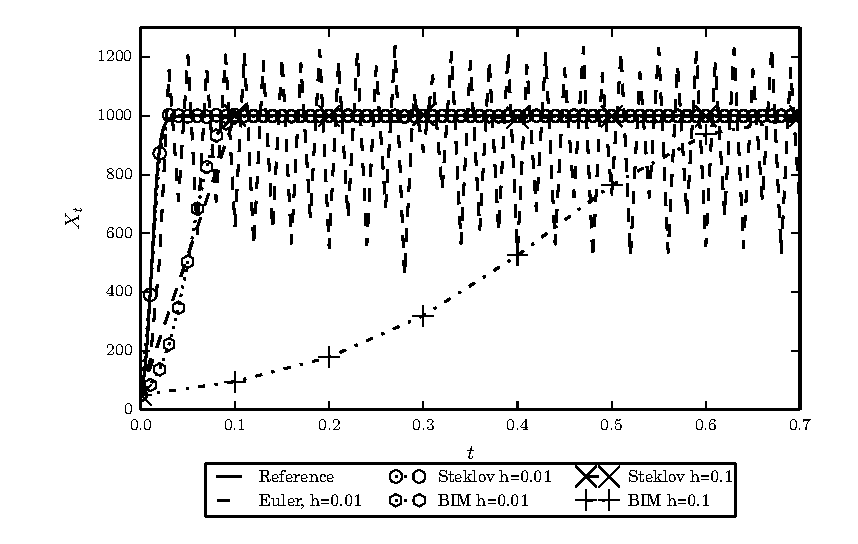
\includegraphics{./papers/paperA/figures/fig1.eps}
    \caption{
      Paths obtained with the Euler, Steklov and BIM methods for the logistic SDE 
      \eqref{eqn:SDELogistic} with $X_0=50$ and taking $K=1000$,
      $\alpha=1$, $\beta$=0.5, $\lambda$=0.25, $\rho=0$ and $\sigma$=$\num{0.05}$.%
    }\label{fig:PathsEDELog}%
  \end{figure}
  \subsection{Langevin equation in Brownian dynamics}\label{sec52}
  Finally, we study the Langevin equation (LE)
  \begin{equation*}
      dX_t= -X_t^3dt+
      \xi dB_t, 
  \end{equation*}
    where $X_t$ is the position of a particle at time $t$ which is exposed to
  deterministic and random forces. This   equation is used in Brownian dynamics like a
  benchmark test, see \cite{Braanka1998}.  As in the logistic SDE, the analytical solution
  for the Langevin equation is only obtained under special conditions. The most common
  Brownian dynamics algorithm  is the CBD method of Ermak and  McCammon \cite{Ermak1978}
  which is based on the Euler discretization of the LE. Although this method is easy to
  implement, a small time step size is required, therefore this algorithm  runs in
  relatively small temporal windows. So, to study the  asymptotic behavior of the solution
  of the LE it is convenient to apply methods with good asymptotic stability properties
  and simple structure. Therefore we show the behavior of the Steklov  method defined by
  the function \eqref{psi3} for short-time and long-time dynamics by  computing  the {\it
  self-diffusion} coefficient $D/D_0$ associated to the LE, for details of the derivation
  of this coefficient see  %\cite{Braanka1998, Lowen1993}. In
  figure\ref{fig:PlotXcubicMSD}, we compare the profiles of the Steklov and
  CBD approximations for several step sizes. According to the notation in Brownian
  dynamics, we take Dta=0.00001 as time step size and use 10 000 sample paths to calculate
  the self-diffusion coefficient. The Steklov and  CBD methods have the same behavior at
  short time with small step sizes. However, for step sizes greater than 1 000 Dta the
  Euler method diverges and the Steklov method preserves its numerical stability. Thus, it
  can be used for long-time dynamics with  big step sizes as it is shown in  figure
  \ref{fig:PlotXcubicMSD}.
  \begin{figure}[h!]
    \begin{center}
        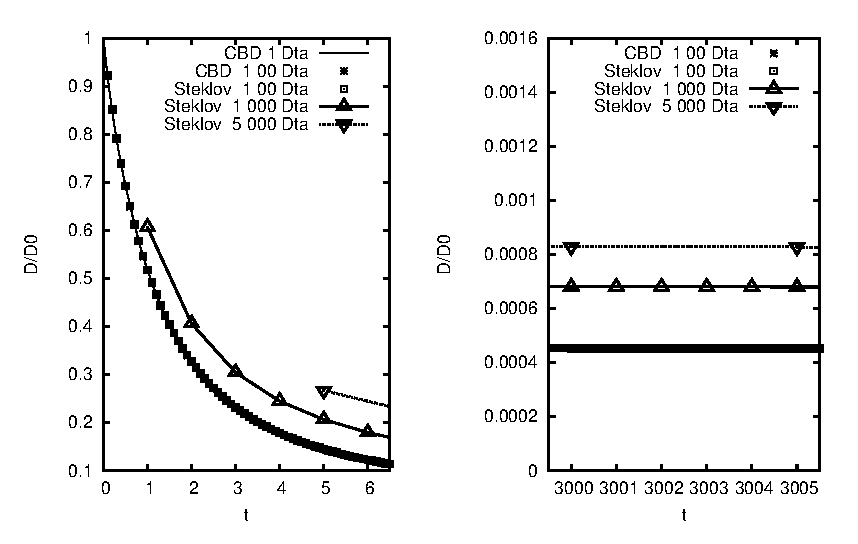
\includegraphics[width= \textwidth]{./papers/paperA/figures/short-longMSD.eps}
    \end{center}
    \caption{
      Numerical results of the Steklov and CBD methods for the self-diffusion coefficient
      of the LE with $\xi=1$: the graph to the left shows short-time simulations and the
      graph to the right  shows long-time simulations. }\label{fig:PlotXcubicMSD}%
  \end{figure}
%%%%%%%%%%%%%%%%%%%%%%%%%%%%%%%%%%%%%%%%%%%%%%%%%%%%%%%%%%%%%%%%%%%%%%%%%%%%%%%%%%%%%%%%%%
%                                 SECTION: Conclusions                                   %
%%%%%%%%%%%%%%%%%%%%%%%%%%%%%%%%%%%%%%%%%%%%%%%%%%%%%%%%%%%%%%%%%%%%%%%%%%%%%%%%%%%%%%%%%%
\section{Conclusions}\label{sec6}
In this paper we have constructed a new method, the explicit Steklov scheme, for the
approximation of stochastic differential equations. We have proved strong consistency and
convergence for this scheme. A linear stability study  of the new scheme has been
performed. Moreover, we give sufficient conditions for the nonlinear asymptotic stability
in both multiplicative and additive cases. Finally, we showed the behavior of the explicit
Steklov method for  problems  with stringent stability requirements as the logistic
stochastic equation and the Langevin equation in Brownian dynamics. In all these studies,
we established that the Steklov method is an accurate scheme for  large time scales
simulation. Future work will focus on the construction and study  of the implicit Steklov
scheme as well as its possible extension to stochastic differential systems.
\appendix
%%%%%%%%%%%%%%%%%%%%%%%%%%%%%%%%%%%%%%%%%%%%%%%%%%%%%%%%%%%%%%%%%%%%%%%%%%%%%%%%%%%%%%%%%%
%                                 BIBLIOGRAPHY                                           %
%%%%%%%%%%%%%%%%%%%%%%%%%%%%%%%%%%%%%%%%%%%%%%%%%%%%%%%%%%%%%%%%%%%%%%%%%%%%%%%%%%%%%%%%%%
%\bibliographystyle{elsarticle-num}
%\bibliography{Bibliography}
% \begin{thebibliography}{30}
% 
% \expandafter\ifx\csname natexlab\endcsname\relax\def\natexlab#1{#1}\fi
% \providecommand{\bibinfo}[2]{#2}
% \ifx\xfnm\relax \def\xfnm[#1]{\unskip,\space#1}\fi
% %Type = Book
% \bibitem[{Allen(2007)}]{EdwardAllen407}
% \bibinfo{author}{E.~Allen}, \bibinfo{title}{{Modeling with It{\^o} Stochastic
%   Differential Equations}}, \bibinfo{publisher}{Springer},
%   \bibinfo{year}{2007}.
% %Type = Book
% \bibitem[{Arnold(1998)}]{LudwigArnold143}
% \bibinfo{author}{L.~Arnold}, \bibinfo{title}{{Random Dynamical Systems}},
%   \bibinfo{publisher}{Springer}, \bibinfo{year}{1998}.
% %Type = Article
% \bibitem[{Baker and Buckwar(2010)}]{Baker2000a}
% \bibinfo{author}{C.T.H. Baker}, \bibinfo{author}{E.~Buckwar},
%   \bibinfo{title}{{Numerical analysis of explicit one-step methods for
%   stochastic delay differential equations}}, \bibinfo{journal}{LMS Journal of
%   Computation and Mathematics} \bibinfo{volume}{3} (\bibinfo{year}{2010})
%   \bibinfo{pages}{315--335}.
% %Type = Article
% \bibitem[{Bokor(2003)}]{Bokor2003}
% \bibinfo{author}{R.H. Bokor}, \bibinfo{title}{{Stochastically stable one-step
%   approximations of solutions of stochastic ordinary differential equations}},
%   \bibinfo{journal}{Applied Numerical Mathematics} \bibinfo{volume}{44}
%   (\bibinfo{year}{2003}) \bibinfo{pages}{299--312}.
% %Type = Article
% \bibitem[{Bra{\'n}ka and Heyes(1998)}]{Braanka1998}
% \bibinfo{author}{A.~Bra{\'n}ka}, \bibinfo{author}{D.~Heyes},
%   \bibinfo{title}{{Algorithms for Brownian dynamics simulation}},
%   \bibinfo{journal}{Physical Review E} \bibinfo{volume}{58}
%   (\bibinfo{year}{1998}) \bibinfo{pages}{2611--2615}.
% %Type = Article
% \bibitem[{Buckwar et~al.(2011)Buckwar, Riedler and Kloeden}]{Buckwar2011a}
% \bibinfo{author}{E.~Buckwar}, \bibinfo{author}{M.G. Riedler},
%   \bibinfo{author}{P.E. Kloeden}, \bibinfo{title}{{The numerical stability of
%   stochastic ordinary differential equations with additive noise}},
%   \bibinfo{journal}{Stochastics and Dynamics} \bibinfo{volume}{11}
%   (\bibinfo{year}{2011}) \bibinfo{pages}{265--281}.
% %Type = Article
% \bibitem[{Burrage et~al.(2004)Burrage, Burrage and Tian}]{Burrage2004}
% \bibinfo{author}{K.~Burrage}, \bibinfo{author}{P.M. Burrage},
%   \bibinfo{author}{T.~Tian}, \bibinfo{title}{{Numerical methods for strong
%   solutions of stochastic differential equations: an overview}},
%   \bibinfo{journal}{Proceedings of the Royal Society A: Mathematical, Physical
%   and Engineering Sciences} \bibinfo{volume}{460} (\bibinfo{year}{2004})
%   \bibinfo{pages}{373--402}.
%  %Type = Article 
% \bibitem[{Bussi y Parrinello(2007)}]{Bussi2007}
% \bibinfo{author}{G.~Bussi}, \bibinfo{author}{M.~Parrinello},
% \bibinfo{title}{{Accurate sampling using Langevin dynamics}},
%  \bibinfo{journal}{Physical Review E} \bibinfo{volume}{75}
% (\bibinfo{year}{2007})  \bibinfo{pages}{056707}.  
% %Type = Article
% \bibitem[{Caraballo and Kloeden(2006)}]{Caraballo2006}
% \bibinfo{author}{T.~Caraballo}, \bibinfo{author}{P.~Kloeden},
%   \bibinfo{title}{{The pathwise numerical approximation of stationary solutions
%   of semilinear stochastic evolution equations}}, \bibinfo{journal}{Applied
%   Mathematics and Optimization} \bibinfo{volume}{54} (\bibinfo{year}{2006})
%   \bibinfo{pages}{401--415}.
% %Type = Article
% \bibitem[{Ermak and a.~McCammon(1978)}]{Ermak1978}
% \bibinfo{author}{D.L. Ermak}, \bibinfo{author}{J.~a.~McCammon},
%   \bibinfo{title}{{Brownian dynamics with hydrodynamic interactions}},
%   \bibinfo{journal}{The Journal of Chemical Physics} \bibinfo{volume}{69}
%   (\bibinfo{year}{1978}) \bibinfo{pages}{1352}.
% %Type = Book
% \bibitem[{Gardiner(2009)}]{gardiner2009stochastic}
% \bibinfo{author}{C.~Gardiner}, \bibinfo{title}{{Stochastic Methods: A Handbook
%   for the Natural and Social Sciences}}, {Springer Series in Synergetics},
%   \bibinfo{publisher}{Springer}, \bibinfo{year}{2009}.
% %Type = Article
% \bibitem[{Hernandez and Spigler(1992)}]{Hernandez1992}
% \bibinfo{author}{D.B. Hernandez}, \bibinfo{author}{R.~Spigler},
%   \bibinfo{title}{{A-stability of Runge-Kutta methods for systems with additive
%   noise}}, \bibinfo{journal}{BIT} \bibinfo{volume}{32} (\bibinfo{year}{1992})
%   \bibinfo{pages}{620--633}.
% %Type = Article
% \bibitem[{Higham(2000{\natexlab{a}})}]{Higham2000}
% \bibinfo{author}{D.J. Higham}, \bibinfo{title}{{A-stability and stochastic
%   mean-square stability}}, \bibinfo{journal}{BIT} \bibinfo{volume}{40}
%   (\bibinfo{year}{2000}{\natexlab{a}}) \bibinfo{pages}{404--409}.
% %Type = Article
% \bibitem[{Higham(2000{\natexlab{b}})}]{Higham2000b}
% \bibinfo{author}{D.J. Higham}, \bibinfo{title}{{Mean-square and asymptotic
%   stability of the stochastic theta method}}, \bibinfo{journal}{SIAM Journal on
%   Numerical Analysis} \bibinfo{volume}{38} (\bibinfo{year}{2000}{\natexlab{b}})
%   \bibinfo{pages}{753--769}.
% %Type = Incollection
% \bibitem[{Kloeden et~al.(1999)Kloeden, Keller and
%   Schmalfu{\ss}}]{kloeden1999towards}
% \bibinfo{author}{P.E. Kloeden}, \bibinfo{author}{H.~Keller},
%   \bibinfo{author}{B.~Schmalfu{\ss}}, \bibinfo{title}{{Towards a Theory of
%   Random Numerical Dynamics}}, in: \bibinfo{editor}{H.~Crauel},
%   \bibinfo{editor}{M.~Gundlach} (Eds.), \bibinfo{booktitle}{{Stochastic
%   Dynamics}}, \bibinfo{publisher}{Springer New York}, \bibinfo{year}{1999}, pp.
%   \bibinfo{pages}{259--282}.
% %Type = Book
% \bibitem[{Kloeden and Platen(1992)}]{PeterE.Kloeden370}
% \bibinfo{author}{P.E. Kloeden}, \bibinfo{author}{E.~Platen},
%   \bibinfo{title}{{Numerical Solution of Stochastic Differential Equations}},
%   \bibinfo{publisher}{Springer-Verlag}, \bibinfo{year}{1992}.
% %Type = Article
% \bibitem[{Lowen and Szamel(1993)}]{Lowen1993}
% \bibinfo{author}{H.~Lowen}, \bibinfo{author}{G.~Szamel},
%   \bibinfo{title}{{Long-time self-diffusion coefficient in colloidal
%   suspensions: theory versus simulation}}, \bibinfo{journal}{Journal of
%   Physics: Condensed Matter} \bibinfo{volume}{5} (\bibinfo{year}{1993})
%   \bibinfo{pages}{2295--2306}.
% %Type = Article
% \bibitem[{Matus et~al.(2005)Matus, Irkhin and
%   Lapinska-Chrzczonowicz}]{Matus2005}
% \bibinfo{author}{P.~Matus}, \bibinfo{author}{U.~Irkhin},
%   \bibinfo{author}{M.~Lapinska-Chrzczonowicz}, \bibinfo{title}{{Exact
%   difference schemes for time-dependent problems}},
%   \bibinfo{journal}{Computational Methods in Applied Mathematics}
%   \bibinfo{volume}{5} (\bibinfo{year}{2005}) \bibinfo{pages}{422--448}.
% %Type = Article
% \bibitem[{Milstein et~al.(1998)Milstein, Platen and Schurz}]{Milstein1998a}
% \bibinfo{author}{G.~Milstein}, \bibinfo{author}{E.~Platen},
%   \bibinfo{author}{H.~Schurz}, \bibinfo{title}{{Balanced implicit methods for
%   stiff stochastic systems}}, \bibinfo{journal}{SIAM Journal on Numerical
%   Analysis} \bibinfo{volume}{35} (\bibinfo{year}{1998})
%   \bibinfo{pages}{1010--1019}.
% %Type = Article
% \bibitem[{Milstein(2003)}]{Milstein2003}
% \bibinfo{author}{G.N. Milstein}, \bibinfo{title}{{Quasi-symplectic methods for
%   Langevin-type equations}}, \bibinfo{journal}{IMA Journal of Numerical
%   Analysis} \bibinfo{volume}{23} (\bibinfo{year}{2003})
%   \bibinfo{pages}{593--626}.
% %Type = Article
% \bibitem[{Pasquali(2001)}]{Pasquali2001}
% \bibinfo{author}{S.~Pasquali}, \bibinfo{title}{{The stochastic logistic
%   equation: stationary solutions and their stability}},
%   \bibinfo{journal}{Rendiconti del Seminario Matematico della Universit{\`a} di
%   Padova} \bibinfo{volume}{106} (\bibinfo{year}{2001})
%   \bibinfo{pages}{165--183}.
% %Type = Article
% \bibitem[{Robinson(2002)}]{Robinson2002}
% \bibinfo{author}{J.C. Robinson}, \bibinfo{title}{{Stability of random
%   attractors under perturbation and approximation}}, \bibinfo{journal}{Journal
%   of Differential Equations} \bibinfo{volume}{186} (\bibinfo{year}{2002})
%   \bibinfo{pages}{652--669}.
% %Type = Article
% \bibitem[{Saito and Mitsui(1996)}]{Saito1996a}
% \bibinfo{author}{Y.~Saito}, \bibinfo{author}{T.~Mitsui},
%   \bibinfo{title}{{Stability analysis of numerical schemes for stochastic
%   differential equations}}, \bibinfo{journal}{SIAM Journal on Numerical
%   Analysis} \bibinfo{volume}{33} (\bibinfo{year}{1996})
%   \bibinfo{pages}{2254--2267}.
% %Type = Article
% \bibitem[{Schurz(2007)}]{Schurz2007}
% \bibinfo{author}{H.~Schurz}, \bibinfo{title}{{Modeling, analysis and
%   discretization of stochastic logistic equations}},
%   \bibinfo{journal}{International Journal of Numerical Analysis and Modeling}
%   \bibinfo{volume}{4} (\bibinfo{year}{2007}) \bibinfo{pages}{178--197}.
% %Type = Article
% \bibitem[{Sun and Wang(2008)}]{Sun2008}
% \bibinfo{author}{X.~Sun}, \bibinfo{author}{Y.~Wang}, \bibinfo{title}{{Stability
%   analysis of a stochastic logistic model with nonlinear diffusion term}},
%   \bibinfo{journal}{Applied Mathematical Modelling} \bibinfo{volume}{32}
%   (\bibinfo{year}{2008}) \bibinfo{pages}{2067--2075}.
% %Type = Book
% \bibitem[{Timan(1963)}]{A.F.Timan65}
% \bibinfo{author}{A.F. Timan}, \bibinfo{title}{{Theory of Approximation of
%   Functions of a Real Variable}}, \bibinfo{publisher}{Dover Publications},
%   \bibinfo{year}{1963}.
% %Type = Book
% \bibitem[{{Van Kampen}(1992)}]{van1992stochastic}
% \bibinfo{author}{N.~{Van Kampen}}, \bibinfo{title}{{Stochastic Processes in
%   Physics and Chemistry}}, {North-Holland Personal Library},
%   \bibinfo{publisher}{Elsevier Science}, \bibinfo{year}{1992}.
% %Type = Book
% \bibitem[{Williams(1991)}]{williams1991probability}
% \bibinfo{author}{D.~Williams}, \bibinfo{title}{{Probability with Martingales}},
%   \bibinfo{publisher}{Cambridge University Press}, \bibinfo{year}{1991}.
% \end{thebibliography}
%\end{document}
